\documentclass[../main]{subfiles}
\ifSubfilesClassLoaded{\setcounter{chapter}{4}}{}
\begin{document}

\chapter{Block Cipher dan Kriptografi Simetris}

\begin{subcpmk}
  \item Sub-CPMK 4.1: Menjelaskan struktur AES dan DES serta mode operasi block cipher (ECB, CBC)
\end{subcpmk}

% ============================================================
% MATERI POKOK
% ============================================================
\section{Pengantar Block Cipher dan DES}

\subsection{Block Cipher}

Block cipher memecah plaintext menjadi blok-blok dengan ukuran tetap, kemudian mengenkripsi setiap blok secara independen. Berbeda dengan cipher klasik yang memproses karakter satu per satu, block cipher bekerja pada unit data yang lebih besar, memberikan keamanan dan efisiensi yang lebih baik. DES adalah contoh paling terkenal dari block cipher yang menggunakan blok 64 bit dengan kunci 56 bit efektif.

DES dikembangkan oleh IBM pada 1970-an dan distandarisasi sebagai FIPS 46 oleh NIST pada 1977 \cite{fips46_3}. Block cipher modern seperti AES menggunakan blok 128 bit dan kunci hingga 256 bit \cite{stallings2017}.

\subsection{Struktur Feistel DES}

DES menggunakan struktur Feistel dengan 16 round untuk menciptakan kebingungan yang tinggi (confusion dan diffusion). Setiap round terdiri dari empat operasi utama: Expansion, Substitution, Permutation, dan Mixing. Struktur ini dirancang untuk memastikan bahwa perubahan kecil dalam plaintext atau kunci akan menyebabkan perubahan besar dalam ciphertext, membuat analisis kriptografi menjadi sangat sulit.

Struktur Feistel memberikan confusion dan diffusion \cite{stallings2017}. Dekripsi mirip enkripsi karena operasi $F$ tidak harus invertible.

\subsection{Fungsi Round DES}

Setiap round DES menggunakan fungsi round yang sama dengan kunci subround yang berbeda. Fungsi ini menggabungkan empat operasi dasar: Expansion E, Substitution S, Permutation P, dan Mixing M. Operasi-operasi ini dirancang untuk memberikan kombinasi optimal antara keamanan dan efisiensi, dengan setiap operasi berkontribusi pada sifat confusion dan diffusion yang diinginkan.

Fungsi round DES memadukan expansion (E), S-box (S), permutation (P) \cite{fips46_3}. Kombinasi ini menciptakan avalanche effect.

\begin{figure}[htbp]
  \centering
  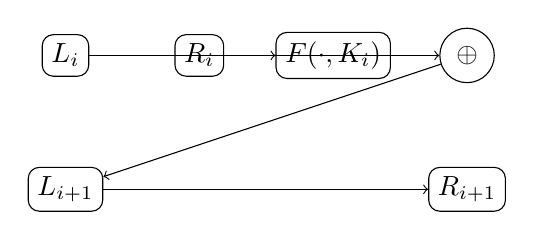
\begin{tikzpicture}[node distance=1.7cm]
    \node (l0) [draw, rounded corners] {$L_i$};
    \node (r0) [draw, rounded corners, right of=l0] {$R_i$};
    \node (f) [draw, rounded corners, right of=r0] {$F(\cdot, K_i)$};
    \node (xor) [draw, circle, right of=f] {$\oplus$};
    \node (l1) [draw, rounded corners, below of=l0] {$L_{i+1}$};
    \node (r1) [draw, rounded corners, below of=xor] {$R_{i+1}$};
    \draw[->] (l0) -- (f);
    \draw[->] (r0) -- (xor);
    \draw[->] (xor) -- (l1);
    \draw[->] (l1) -- (r1);
  \end{tikzpicture}
  \caption{Satu putaran Feistel DES.}
\end{figure}

\begin{lstlisting}[style=cstyle, caption={Satu putaran Feistel (pseudocode)}]
void des_round(uint32_t *L, uint32_t *R, uint32_t *K, uint32_t round) {
    // Expansion E: 32 bit -> 48 bit
    uint64_t expanded_R = expand_e(R[round]);
    
    // Substitution S: 48 bit -> 48 bit
    uint32_t substituted_R = substitution_s(expanded_R, K[round]);
    
    // Permutation P: 48 bit -> 48 bit
    uint32_t permuted_R = permutation_p(substituted_R);
    
    // Mixing: 48 bit -> 32 bit
    uint32_t mixed_R = mixing_m(permuted_R);
    
    // XOR dengan subkey
    R[round + 1] = mixed_R ^ K[round];
}
\end{lstlisting}

\subsection{Fungsi dan Komponen DES}

DES memiliki beberapa komponen fundamental yang bekerja sama untuk menciptakan keamanan tinggi. Initial Permutation (IP) mengacak urutan 64 bit plaintext sebelum enkripsi, sedangkan Final Permutation (FP) mengacak kembali setelah 16 round. S-box (Substitution Box) melakukan substitusi non-linear 6 bit ke 4 bit, menciptakan kebingungan yang sangat kompleks dan sulit dianalisis tanpa mengetahui desain internalnya.

\begin{table}[htbp]
  \centering
  \small
  \begin{tabular}{lll}
    \toprule
    Komponen & Fungsi & Ukuran \\
    \midrule
    Initial Permutation & Mengacak bit plaintext & 64 bit \\
    Expansion Function & Menambah 16 bit ke 48 bit & 32→48 bit \\
    S-box & Substitusi non-linear 6→4 bit & 6→4 bit (8 kotak) \\
    Permutation & Mengacak posisi bit & 32 bit \\
    Key Schedule & Menghasilkan 16 subkunci & 56→64 bit \\
    \bottomrule
  \end{tabular}
  \caption{Komponen utama DES dan fungsinya.}
\end{table}

\subsection{DES (Data Encryption Standard)}

DES distandarisasi sebagai FIPS 46 oleh NIST \cite{fips46_3}. Blok 64 bit, kunci 56 bit efektif. Kerentanan utama: brute force (56 bit) dan differential/linear cryptanalysis \cite{stallings2017}.

\subsection{Serangan terhadap DES}

DES rentan terhadap brute force (kunci 56 bit dapat dipecahkan dalam waktu wajar), differential cryptanalysis, dan linear cryptanalysis \cite{menezes1996}.

\subsection{3DES (Triple DES)}

3DES menerapkan DES tiga kali dengan kunci berbeda; keamanan efektif sekitar 112 bit \cite{stallings2017}. 3DES lebih lambat; untuk aplikasi baru gunakan AES.

\begin{table}[htbp]
  \centering
  \small
  \begin{tabular}{lcc}
    \toprule
    Metode & Keamanan & Performa \\
    \midrule
    DES & Standar, kunci pendek & Cepat \\
    3DES & Lebih aman, kunci panjang & Lebih lambat \\
    \bottomrule
  \end{tabular}
  \caption{Perbandingan DES dan 3DES.}
\end{table}

\subsection{Implementasi Praktis}

Implementasi DES hanya direkomendasikan untuk tujuan edukasi. Gunakan library teruji (OpenSSL, libsodium) untuk produksi \cite{ferguson2010}.

\begin{catatan}
Implementasi manual DES hanya direkomendasikan untuk tujuan edukasi dan pemahaman konsep. Untuk aplikasi produksi, selalu gunakan library yang telah melalui audit keamanan profesional dan validasi standar industri. Hindari implementasi sendiri dari algoritma kompleks seperti DES kecuali jika diperlukan untuk pembelajaran mendalam tentang kriptanalisis.
\end{catatan}

\subsection{Key Schedule DES}

Kunci DES 64 bit mengandung 8 bit parity, sehingga hanya 56 bit efektif. Proses key schedule:
\begin{itemize}
  \item \textbf{PC-1}: pilih 56 bit dan bagi menjadi $C_0$ dan $D_0$ (masing-masing 28 bit).
  \item \textbf{Left shift}: $C_i$ dan $D_i$ digeser 1 atau 2 bit sesuai tabel.
  \item \textbf{PC-2}: pilih 48 bit dari gabungan $C_i||D_i$ menjadi subkey $K_i$.
\end{itemize}

\begin{table}[htbp]
  \centering
  \small
  \begin{tabular}{cccccccc}
    \toprule
    Round & 1 & 2 & 3 & 4 & 5 & 6 & 7 \\
    Shift & 1 & 1 & 2 & 2 & 2 & 2 & 2 \\
    \midrule
    Round & 8 & 9 & 10 & 11 & 12 & 13 & 14 \\
    Shift & 2 & 1 & 2 & 2 & 2 & 2 & 2 \\
    \midrule
    Round & 15 & 16 & & & & & \\
    Shift & 2 & 1 & & & & & \\
    \bottomrule
  \end{tabular}
  \caption{Jadwal pergeseran kunci DES.}
\end{table}

\subsection{Serangan terhadap DES dan 3DES}

\begin{itemize}
  \item \textbf{Brute force}: 56-bit key dapat dipecahkan dengan perangkat modern.
  \item \textbf{Differential/linear cryptanalysis}: teknik analitis terhadap struktur DES.
  \item \textbf{3DES}: lebih aman tetapi lebih lambat; rentan \textit{meet-in-the-middle} dengan keamanan efektif sekitar 112 bit \cite{stallings2017}.
\end{itemize}

\subsection{Evolusi dari DES ke AES}

AES dipilih NIST (1997--2000) sebagai pemenang kompetisi; Rijndael menang \cite{fips197}. AES menggunakan blok 128 bit, kunci 128/192/256 bit.

\subsection{Pentingnya DES dalam Sejarah Kriptografi}

DES adalah cipher simetris pertama yang distandarisasi publik; konsep S-box, Feistel, confusion/diffusion tetap fundamental \cite{stallings2017}.

\begin{catatan}
Studi DES tetap penting untuk pemahaman mendalam tentang kriptografi simetris dan kriptanalisis. Banyak konsep fundamental dalam kriptografi modern, seperti confusion, diffusion, dan avalanche effect, pertama kali dipelajari secara mendalam melalui analisis DES. Meskipun tidak lagi digunakan dalam produksi, DES tetap menjadi alat edukasi yang sangat berharga.
\end{catatan}

\section{AES (Advanced Encryption Standard)}

\subsection{Overview}

AES menggantikan DES sebagai standar enkripsi simetris modern. Dipilih melalui kompetisi NIST (1997--2000), pemenangnya Rijndael \cite{nist}. AES menggunakan blok 128 bit dan kunci 128, 192, atau 256 bit. Menurut Wikipedia, AES didasarkan pada desain substitution-permutation network yang efisien baik dalam perangkat lunak maupun perangkat keras.

AES dikembangkan oleh dua kriptografer Belgia, Joan Daemen dan Vincent Rijmen, dari Katholieke Universiteit Leuven. Menurut Wikipedia, Rijndael diumumkan sebagai pemenang kompetisi AES pada Oktober 2000 setelah melalui evaluasi ketat dari 15 kandidat algoritma. Algoritma ini dipilih karena keunggulannya dalam keamanan, efisiensi, fleksibilitas implementasi, dan kesederhanaan desain matematisnya.

\subsection{Struktur AES}

AES bukan Feistel. Setiap round terdiri dari:
\begin{itemize}
  \item \textbf{SubBytes}: Substitusi byte dengan S-box
  \item \textbf{ShiftRows}: Menggeser baris state
  \item \textbf{MixColumns}: Operasi linear pada kolom
  \item \textbf{AddRoundKey}: XOR dengan subkey
\end{itemize}

Jumlah round: 10 (kunci 128 bit), 12 (192 bit), 14 (256 bit).

Struktur AES menggunakan substitution-permutation network yang berbeda dari struktur Feistel DES. Menurut Wikipedia, setiap operasi AES dirancang untuk memberikan kombinasi optimal dari confusion (melalui SubBytes) dan diffusion (melalui ShiftRows dan MixColumns). Operasi ini bekerja pada finite field \(\mathrm{GF}(2^{8})\) yang memastikan sifat matematis yang kuat dan dapat dibuktikan keamanannya.

\subsection{State dan Urutan Round}

AES bekerja pada \textbf{state} 4x4 byte (128 bit). Byte plaintext diisikan kolom demi kolom:
\begin{table}[htbp]
  \centering
  \small
  \begin{tabular}{cccc}
    \toprule
    $b_0$ & $b_4$ & $b_8$ & $b_{12}$ \\
    $b_1$ & $b_5$ & $b_9$ & $b_{13}$ \\
    $b_2$ & $b_6$ & $b_{10}$ & $b_{14}$ \\
    $b_3$ & $b_7$ & $b_{11}$ & $b_{15}$ \\
    \bottomrule
  \end{tabular}
  \caption{Representasi state AES (kolom per kolom).}
\end{table}

Urutan round AES-128 \cite{fips197}:
\begin{enumerate}
  \item \textbf{Initial AddRoundKey}
  \item 9 round: SubBytes $\rightarrow$ ShiftRows $\rightarrow$ MixColumns $\rightarrow$ AddRoundKey
  \item Final round: SubBytes $\rightarrow$ ShiftRows $\rightarrow$ AddRoundKey (tanpa MixColumns)
\end{enumerate}

Representasi state AES sangat penting untuk implementasi yang efisien. Menurut Wikipedia, state disusun dalam column-major order yang memungkinkan operasi MixColumns dilakukan secara optimal pada setiap kolom. Struktur 4x4 byte ini juga memfasilitasi implementasi perangkat keras yang efisien dan operasi parallel pada prosesor modern.

\subsection{Operasi Detil AES}

\subsubsection{SubBytes}
SubBytes melakukan substitusi non-linear pada setiap byte state menggunakan S-box AES yang sama untuk semua round. Menurut Wikipedia, S-box AES dirancang untuk memberikan sifat confusion yang kuat dan resistensi terhadap differential cryptanalysis. S-box ini dibangun menggunakan inversi multiplicative di finite field \(\mathrm{GF}(2^{8})\) diikuti dengan transformasi affine yang dipilih secara hati-hati.

\subsubsection{ShiftRows}
ShiftRows menggeser setiap baris state dengan jumlah yang berbeda: baris pertama tidak digeser, baris kedua digeser 1 byte ke kiri, baris ketiga digeser 2 byte, dan baris keempat digeser 3 byte. Menurut Wikipedia, operasi ini menyebarkan pengaruh setiap byte ke kolom yang berbeda, menciptakan efek diffusion yang penting untuk keamanan.

\subsubsection{MixColumns}
MixColumns melakukan operasi linear pada setiap kolom state menggunakan matriks tetap di finite field \(\mathrm{GF}(2^{8})\). Menurut Wikipedia, operasi ini memastikan bahwa perubahan kecil pada input akan menyebabkan perubahan besar pada output, menciptakan sifat avalanche yang sangat penting. MixColumns tidak diterapkan pada round terakhir untuk memfasilitasi implementasi yang simetris untuk enkripsi dan dekripsi.

\subsubsection{AddRoundKey}
AddRoundKey melakukan XOR antara state dan round key yang sesuai. Menurut Wikipedia, operasi ini adalah satu-satunya operasi dalam AES yang bergantung pada kunci, memastikan bahwa tanpa kunci yang benar, semua operasi lain tidak dapat dibalik. Round key dihasilkan dari key schedule yang kompleks untuk mencegah serangan related-key.

\subsection{Key Schedule AES}

AES-128 menghasilkan 11 round key (44 word). Proses kunci \cite{fips197}:
\begin{itemize}
  \item \textbf{RotWord}: rotasi 1 byte.
  \item \textbf{SubWord}: substitusi S-box.
  \item \textbf{Rcon}: konstanta round.
\end{itemize}
Secara ringkas, untuk setiap word $w_i$:
\[
w_i =
\begin{cases}
w_{i-4} \oplus \text{SubWord}(\text{RotWord}(w_{i-1})) \oplus \text{Rcon} & i \equiv 0 \pmod{4} \\
w_{i-4} \oplus w_{i-1} & \text{lainnya}
\end{cases}
\]

\begin{table}[htbp]
  \centering
  \small
  \begin{tabular}{cccc}
    \toprule
    Rcon[1] & Rcon[2] & Rcon[3] & Rcon[4] \\
    \midrule
    01 & 02 & 04 & 08 \\
    \bottomrule
  \end{tabular}
  \caption{Contoh konstanta Rcon (hex) untuk AES-128.}
\end{table}

Key schedule AES dirancang untuk mencegah serangan related-key dan weak keys. Menurut Wikipedia, proses ini menghasilkan 44 word untuk AES-128, 52 word untuk AES-192, dan 60 word untuk AES-256, memberikan distribusi kunci yang merata di semua round. Penggunaan Rcon yang berbeda untuk setiap 4 word memastikan bahwa tidak ada pola kunci yang dapat dieksploitasi.

\subsection{Keamanan AES}

AES dianggap aman terhadap serangan known-plaintext dan chosen-plaintext. Implementasi praktis biasanya menggunakan library (misalnya OpenSSL) karena kompleksitas dan risiko kesalahan implementasi manual. Menurut Wikipedia, AES telah melalui evaluasi keamanan ekstensif dan tidak ditemukan kerentanan praktis hingga saat ini.

\begin{catatan}
Keamanan AES dapat runtuh jika implementasi bocor melalui \textit{side-channel} (timing, cache). Gunakan library yang sudah teruji dan hindari implementasi manual yang tidak \textit{constant-time} \cite{ferguson2010}.
\end{catatan}

\subsection{Implementasi dan Optimasi}

Implementasi AES dapat dioptimasi untuk berbagai platform dengan teknik yang berbeda. Menurut Wikipedia, implementasi perangkat lunak modern menggunakan tabel lookup (T-tables) untuk menggabungkan SubBytes, ShiftRows, dan MixColumns dalam satu operasi, meningkatkan kecepatan secara signifikan. Implementasi perangkat keras menggunakan sirkuit khusus untuk operasi finite field yang sangat efisien.

\begin{table}[htbp]
  \centering
  \small
  \begin{tabular}{lcc}
    \toprule
    Metode Implementasi & Kecepatan & Penggunaan Memori \\
    \midrule
    Naive & Lambat & Rendah \\
    T-tables & Cepat & Sedang \\
    Bitslicing & Sangat Cepat & Tinggi \\
    Hardware & Paling Cepat & Rendah \\
    \bottomrule
  \end{tabular}
  \caption{Perbandingan metode implementasi AES.}
\end{table}

\section{Mode Operasi Block Cipher}

Block cipher mengenkripsi satu blok. Untuk data lebih panjang, digunakan \textbf{mode operasi}. Mode operasi sangat penting karena menentukan bagaimana block cipher digunakan untuk mengenkripsi data yang lebih panjang dari satu blok, serta mempengaruhi keamanan dan efisiensi implementasi.

Mode operasi block cipher berevolusi dari waktu ke waktu untuk mengatasi berbagai kelemahan keamanan. Menurut Wikipedia, mode-mode paling awal seperti ECB, CBC, OFB, dan CFB telah ada sejak tahun 1981 dan distandarisasi dalam FIPS 81. Seiring waktu, mode baru seperti CTR dan GCM dikembangkan untuk mengatasi kelemahan mode-mode sebelumnya dan menyediakan fitur tambahan seperti autentikasi.

\subsection{ECB (Electronic Codebook)}

Setiap blok dienkripsi independen. \textbf{Kelemahan}: Blok plaintext identik menghasilkan ciphertext identik—rentan analisis pola. Tidak direkomendasikan untuk data sensitif. Menurut Wikipedia, ECB adalah mode yang paling sederhana tetapi juga paling tidak aman karena tidak menyediakan semantic security dan sangat rentan terhadap serangan pattern analysis.

ECB memiliki kelemahan fundamental yang sangat serius dalam aplikasi praktis. Menurut sumber keamanan, ECB tidak menyediakan semantic security karena plaintext identik menghasilkan ciphertext identik, yang sangat berbahaya untuk data terstruktur seperti gambar atau dokumen terformat. Mode ini hanya cocok untuk enkripsi data acak yang sangat pendek atau sebagai komponen dalam protokol yang lebih kompleks.

\subsection{CBC (Cipher Block Chaining)}

Setiap blok plaintext di-XOR dengan ciphertext blok sebelumnya sebelum enkripsi. Blok pertama di-XOR dengan \textbf{IV} (Initialization Vector). IV harus acak dan unik per enkripsi, dapat dikirim bersama ciphertext. Menurut Wikipedia, CBC adalah mode yang paling umum digunakan sebelum munculnya mode AEAD modern.

CBC menyediakan keamanan yang jauh lebih baik dibandingkan ECB karena setiap blok ciphertext bergantung pada semua blok sebelumnya. Menurut sumber keamanan, IV harus unik untuk setiap enkripsi dengan kunci yang sama untuk mencegah serangan replay dan memastikan semantic security. Namun, CBC tidak dapat diparalelkan selama enkripsi dan rentan terhadap padding oracle attacks.

\subsection{Padding (PKCS\#7)}

Jika panjang plaintext tidak kelipatan ukuran blok, digunakan padding. PKCS\#7 menambah $k$ byte bernilai $k$ (1--block size) \cite{rfc5652}:
\begin{itemize}
  \item Jika blok sisa 5 byte pada AES (16 byte), tambahkan 11 byte bernilai 0x0B.
  \item Jika plaintext tepat kelipatan blok, tambahkan satu blok penuh bernilai 0x10.
\end{itemize}

Padding PKCS\#7 adalah standar industri yang digunakan secara luas dalam implementasi CBC dan mode-mode lainnya. Menurut RFC 5652, padding ini dirancang untuk dapat dihapus secara unik setelah dekripsi, mencegah ambiguitas dalam menentukan panjang plaintext asli. Namun, implementasi padding yang salah dapat menyebabkan kerentanan padding oracle attacks yang sangat serius.

\begin{catatan}
Pada CBC, padding yang salah dapat memicu \textit{padding oracle} jika pesan kesalahan dibedakan. Gunakan mode AEAD (mis. GCM) untuk integritas \cite{nist800_38d}.
\end{catatan}

\subsection{CFB dan OFB}

CFB (Cipher Feedback) dan OFB (Output Feedback): mengubah block cipher menjadi stream cipher. Keduanya membutuhkan IV. Menurut Wikipedia, CFB dan OFB dikembangkan untuk mengatasi keterbatasan ECB dan CBC, terutama untuk aplikasi yang memerlukan stream cipher atau komunikasi real-time.

CFB dan OFB memiliki karakteristik yang berbeda yang membuatnya cocok untuk aplikasi tertentu. Menurut sumber keamanan, CFB memungkinkan enkripsi data yang tidak kelipatan blok dan dapat pulih dari error bit, sedangkan OFB memberikan stream cipher yang sinkron dan lebih resisten terhadap error propagation. Keduanya memerlukan IV yang unik untuk setiap sesi komunikasi.

\subsection{CTR (Counter Mode)}

CTR membuat \textit{keystream} dengan mengenkripsi nonce||counter, lalu di-XOR dengan plaintext. Mode ini paralel dan tidak memerlukan padding \cite{nist800_38a}. Menurut Wikipedia, CTR menjadi sangat populer karena efisiensinya dan kemampuan untuk diparalelkan, membuatnya ideal untuk implementasi modern pada multi-core processors.

CTR menawarkan keuntungan performa yang signifikan dibandingkan mode-mode lainnya. Menurut sumber keamanan, CTR dapat diimplementasikan secara paralel penuh baik untuk enkripsi maupun dekripsi, dan tidak memerlukan padding karena keystream dapat dipotong sesuai panjang plaintext. Namun, nonce harus unik untuk setiap enkripsi dengan kunci yang sama untuk mencegah keystream reuse.

\subsection{AEAD: GCM/CCM}

GCM dan CCM memberikan kerahasiaan sekaligus integritas (AEAD). Nonce harus unik; reuse nonce pada GCM dapat membocorkan kunci \cite{nist800_38d}. Menurut Wikipedia, AEAD mode menjadi standar modern karena menyederhanakan implementasi keamanan dengan menggabungkan enkripsi dan autentikasi dalam satu operasi atomik.

GCM (Galois/Counter Mode) dan CCM (Counter with CBC-MAC) mewakili evolusi terbaru dalam mode operasi block cipher. Menurut sumber keamanan, GCM menggunakan Galois Field multiplication untuk autentikasi yang sangat efisien dalam perangkat keras, sedangkan CCM menggabungkan CTR untuk enkripsi dengan CBC-MAC untuk autentikasi. Keduanya menyediakan keamanan yang komprehensif dengan overhead minimal.

\subsection{XTS untuk Storage}

XTS dirancang untuk enkripsi disk/penyimpanan, menghindari pola blok berulang pada sektor \cite{nist800_38e}. Menurut Wikipedia, XTS dikembangkan khusus untuk aplikasi penyimpanan data di mana data dapat diubah secara parsial dan memerlukan tweakable encryption untuk mencegah pola yang dapat dieksploitasi.

XTS menggunakan tweakable encryption yang memungkinkan modifikasi data tanpa mengenkripsi ulang seluruh sektor. Menurut sumber keamanan, mode ini menggunakan dua kunci dan sector number sebagai tweak untuk memastikan bahwa sektor yang sama dengan data berbeda menghasilkan ciphertext yang berbeda, mencegah serangan pattern analysis pada sistem penyimpanan.

\subsection{Aturan IV/Nonce}

\begin{itemize}
  \item \textbf{CBC/CFB/OFB}: IV harus acak dan tidak boleh diulang.
  \item \textbf{CTR/GCM/CCM}: nonce harus unik untuk setiap enkripsi dengan kunci yang sama.
\end{itemize}

\begin{figure}[htbp]
  \centering
  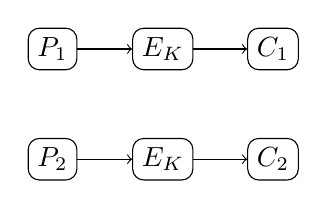
\begin{tikzpicture}[node distance=1.4cm]
    \node (p1) [draw, rounded corners] {$P_1$};
    \node (e1) [draw, rounded corners, right of=p1] {$E_K$};
    \node (c1) [draw, rounded corners, right of=e1] {$C_1$};
    \draw[->] (p1) -- (e1);
    \draw[->] (e1) -- (c1);
    \node (p2) [draw, rounded corners, below of=p1] {$P_2$};
    \node (e2) [draw, rounded corners, right of=p2] {$E_K$};
    \node (c2) [draw, rounded corners, right of=e2] {$C_2$};
    \draw[->] (p2) -- (e2);
    \draw[->] (e2) -- (c2);
  \end{tikzpicture}
  \caption{ECB: tiap blok independen.}
\end{figure}

\begin{figure}[htbp]
  \centering
  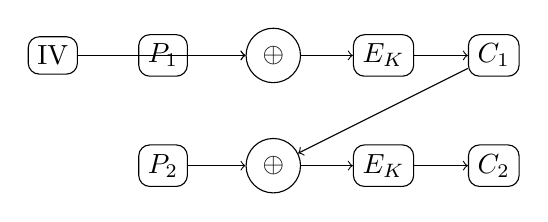
\begin{tikzpicture}[node distance=1.4cm]
    \node (iv) [draw, rounded corners] {IV};
    \node (p1) [draw, rounded corners, right of=iv] {$P_1$};
    \node (xor1) [draw, circle, right of=p1] {$\oplus$};
    \node (e1) [draw, rounded corners, right of=xor1] {$E_K$};
    \node (c1) [draw, rounded corners, right of=e1] {$C_1$};
    \node (p2) [draw, rounded corners, below of=p1] {$P_2$};
    \node (xor2) [draw, circle, right of=p2] {$\oplus$};
    \node (e2) [draw, rounded corners, right of=xor2] {$E_K$};
    \node (c2) [draw, rounded corners, right of=e2] {$C_2$};
    \draw[->] (iv) -- (xor1);
    \draw[->] (p1) -- (xor1);
    \draw[->] (xor1) -- (e1);
    \draw[->] (e1) -- (c1);
    \draw[->] (c1) -- (xor2);
    \draw[->] (p2) -- (xor2);
    \draw[->] (xor2) -- (e2);
    \draw[->] (e2) -- (c2);
  \end{tikzpicture}
  \caption{CBC: blok saling terikat melalui XOR.}
\end{figure}

\begin{figure}[htbp]
  \centering
  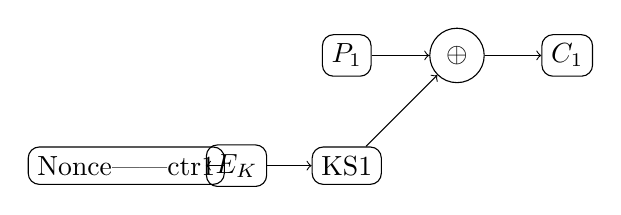
\begin{tikzpicture}[node distance=1.4cm]
    \node (n1) [draw, rounded corners] {Nonce||ctr1};
    \node (e1) [draw, rounded corners, right of=n1] {$E_K$};
    \node (k1) [draw, rounded corners, right of=e1] {KS1};
    \node (p1) [draw, rounded corners, above of=k1] {$P_1$};
    \node (xor1) [draw, circle, right of=p1] {$\oplus$};
    \node (c1) [draw, rounded corners, right of=xor1] {$C_1$};
    \draw[->] (n1) -- (e1);
    \draw[->] (e1) -- (k1);
    \draw[->] (p1) -- (xor1);
    \draw[->] (k1) -- (xor1);
    \draw[->] (xor1) -- (c1);
  \end{tikzpicture}
  \caption{CTR: keystream dari nonce||counter.}
\end{figure}

\subsection{Ringkasan Perbandingan Mode}

\begin{table}[htbp]
  \centering
  \small
  \begin{tabular}{lcccc}
    \toprule
    Mode & Perlu IV/Nonce & Perlu Padding & Paralel (enk) & Integritas \\
    \midrule
    ECB & Tidak & Ya & Ya & Tidak \\
    CBC & Ya & Ya & Tidak & Tidak \\
    CFB/OFB & Ya & Tidak & Sebagian & Tidak \\
    CTR & Ya & Tidak & Ya & Tidak \\
    GCM/CCM & Ya & Tidak & Ya & Ya \\
    \bottomrule
  \end{tabular}
  \caption{Perbandingan singkat mode operasi block cipher.}
\end{table}

\subsection{Contoh Pseudocode (CBC dan CTR)}

\begin{lstlisting}[style=cstyle, caption={CBC encryption (pseudocode)}]
for i = 0..n-1:
    x = P[i] ^ (i==0 ? IV : C[i-1]);
    C[i] = E_K(x);
\end{lstlisting}

\begin{lstlisting}[style=cstyle, caption={CTR encryption (pseudocode)}]
for i = 0..n-1:
    KS = E_K(nonce || counter);
    C[i] = P[i] ^ KS;
    counter++;
\end{lstlisting}

\begin{catatan}
Untuk keamanan, gunakan CBC, CFB, atau OFB dengan IV acak—bukan ECB. AES-CBC dan AES-GCM umum digunakan dalam praktik \cite{ferguson2010}.
\end{catatan}


% ============================================================
% AKTIVITAS PEMBELAJARAN
% ============================================================

\begin{aktivitas}
  \item \textbf{Studi Literatur}: Bandingkan struktur Feistel (DES) dengan struktur AES. Apa perbedaan utama?
  
  \item \textbf{Praktikum}: Gunakan OpenSSL atau library C untuk mengenkripsi file dengan AES-CBC. Amati peran IV.
  
  \item \textbf{Analisis}: Mengapa ECB tidak aman? Cari contoh visual (gambar terenkripsi ECB vs CBC).
\end{aktivitas}

% ============================================================
% LATIHAN DAN REFLEKSI
% ============================================================

\begin{latihan}
  \item Jelaskan struktur Feistel. Mengapa dekripsi Feistel mirip dengan enkripsi?
  
  \item Sebutkan 4 operasi dalam satu round AES.
  
  \item Jelaskan perbedaan ECB dan CBC. Mengapa CBC lebih aman?
  
  \item Apa fungsi IV dalam mode CBC?
\end{latihan}

% ============================================================
% ASESMEN
% ============================================================

\begin{asesmen}
\textbf{Instrumen Penilaian untuk Sub-CPMK 4.1}

Jelaskan dalam bentuk essay: (a) Mengapa DES tidak lagi aman? (b) Apa keunggulan AES dibanding DES? (c) Kapan mode ECB masih dapat digunakan?
\end{asesmen}

% ============================================================
% CHECKLIST KOMPETENSI
% ============================================================

\begin{checklist}
  \item Saya dapat menjelaskan struktur DES (Feistel)
  \item Saya dapat menjelaskan struktur AES (SubBytes, ShiftRows, MixColumns, AddRoundKey)
  \item Saya dapat membedakan mode ECB, CBC, CFB, OFB
  \item Saya memahami peran IV dalam mode CBC
\end{checklist}

% ============================================================
% RANGKUMAN
% ============================================================

\begin{rangkuman}
Bab ini membahas block cipher DES dan AES, serta mode operasi ECB, CBC, CFB, OFB. AES adalah standar modern untuk enkripsi simetris.

\textbf{Poin Kunci:}
\begin{itemize}
  \item DES: Feistel, 64-bit block, 56-bit key; tidak aman untuk aplikasi baru
  \item AES: blok 128 bit, kunci 128/192/256 bit; standar NIST
  \item Mode operasi: ECB (lemah), CBC/CFB/OFB (lebih aman dengan IV)
\end{itemize}

\textbf{Kata Kunci}: \crypt{Block Cipher}, \crypt{DES}, \crypt{AES}, \crypt{Feistel}, \crypt{ECB}, \crypt{CBC}
\end{rangkuman}

\ifSubfilesClassLoaded{
  \renewcommand{\bibname}{Daftar Pustaka}
  \bibliographystyle{plain}
  \bibliography{../references}
}{}
\end{document}
